\documentclass[article,dr=phil,type=drfinal,colorback,accentcolor=tud9c]{tudthesis}
%\usepackage{ngerman}
\usepackage{tikz}
\usepackage{pgfplots}
\usepackage{pdfpages}
\usepackage{subfig}
\usepackage{graphicx}
\usepackage{ctable}
\usepackage{multirow}
\usepackage{tabularx}
\usepackage{algorithm2e}
\usepackage[noend]{algpseudocode}






% Farbpalette A
\definecolor{blau_1a}{RGB}{93,133,195}
\definecolor{blau_2a}{RGB}{0,156,218}
\definecolor{gruen_3a}{RGB}{80,182,149}
\definecolor{gruen_4a}{RGB}{175,204,80}
\definecolor{gruen_5a}{RGB}{221,223,72}
\definecolor{orange_6a}{RGB}{255,224,92}
\definecolor{orange_7a}{RGB}{248,186,60}
\definecolor{rot_8a}{RGB}{238,122,52}
\definecolor{rot_9a}{RGB}{233,80,62}
\definecolor{lila_10a}{RGB}{201,48,142}
\definecolor{lila_11a}{RGB}{128,69,151}

% Farbpalette B
\definecolor{blau_1b}{RGB}{0,90,169}
\definecolor{blau_2b}{RGB}{0,131,204}
\definecolor{gruen_3b}{RGB}{0,157,129}
\definecolor{gruen_4b}{RGB}{153,192,0}
\definecolor{gruen_5b}{RGB}{201,212,0}
\definecolor{orange_6b}{RGB}{253,202,0}
\definecolor{orange_7b}{RGB}{245,163,0}
\definecolor{rot_8b}{RGB}{236,101,0}
\definecolor{rot_9b}{RGB}{230,0,26}
\definecolor{lila_10b}{RGB}{166,0,132}
\definecolor{lila_11b}{RGB}{114,16,133}
\newcommand{\getmydate}{%
  \ifcase\month%
    \or Januar\or Februar\or M\"arz%
    \or April\or Mai\or Juni\or Juli%
    \or August\or September\or Oktober%
    \or November\or Dezember%
  \fi\ \number\year%
}

\begin{document}
  \thesistitle{Parallel word sense disambigation of Hyperlex Algorithm}%
    {Parallel word sense disambigation of Hyperlex Algorithm}
  \author{Viswanath Vadhri}
  \birthplace{Darmstadt}
  \referee{Prof. Dr. Felix Wolf}{Sebastian Rinke}
  \department{Fachbereich Informatik}
  \group{Laboratory for Parallel Programming}
  \dateofexam{\today}{\today}
  \tuprints{12345}{1234}
  \makethesistitle
  \affidavit{V. Vadhri}

\newpage
\begin{abstract}
Word sense disambiguation (WSD) is the ability to identify the intended meanings of words (word senses) in a context. It is a central research topic in Natural Language Processing (NLP). Word sense disambiguation is often characterized as an intermediate task, which is not an end in itself, but essential for many applications requiring broad-coverage language understanding. Examples include machine translation, information retrieval, information extraction or text mining.

Hyperlex is an unsupervised graph-based technique used in Natural Language Processing that is capable of automatically determining word senses from a large text base without recourse to a dictionary with excellent precision. In this thesis, we design and implement the Hyperlex algorithm as a scalable application which runs on the cluster and can process data of magnitude Terabytes. We analyse the results of the implementation.


\end{abstract}


\newpage
\tableofcontents

\newpage
\chapter{}
  \section{Introduction}
  Word sense disambiguation is about automatically recognizing which of multiple meanings of ambiguous words is being used in a specific sentence. Words have different properties one of them is polysemy. Polysemy means many words have multiple senses. Here is an example 'Lets have a drink in the bar'. The word bar in this sentence means a drinking establishment, however in general the word bar has many other meanings. so for example 'bring me a chocalate bar'. 'I have to study for the bar', the meaning of bar in this case it means some exam for lawyers.

Lets have a drink in the bar
Bring me a chocolate bar.
I have to study for the bar.

Here are a few meanings taken from the wordnet dictionary for the word 'bar'

\begin{enumerate}
  \item barroom, bar, saloon, ginmill, taproom - a room or establishment where alcoholic drinks are served over a counter; "he drowned his sorrows in whiskey at the bar"
  \item bar - a counter where you can obtain food or drink; "he bought a hot dog and a coke at the bar"
  \item prevention, bar - the act of preventing; "there was no bar against leaving"; "money was allocated to study the cause and prevention of influenza"
  \item legal profession, bar, legal community - the body of individuals qualified to practice law in a particular jurisdiction; "he was admitted to the bar in New Jersey"
\end{enumerate}


So the main goal of WSD here is to take a word like bar that has multiple senses and then in a given sentence findout which of those meanings is being used. So we need have the entire context, so we typically get access to the entire sentence and often to the entire paragraph in which the word appears.


  \subsection{Application}
    Word sense disambiguation is very important component of Natural Language processing systems because its used for example to come up with for example semantic representations of sentences and also for question-answering and for things like maching translation. Obviously if a word is ambiguous in one language it doesnt necessarily mean it is also ambiguous in another language. So for example if we want to translate the word 'play' from English to Spanish. We need to understand what is the object being played, so for example in english we say 'play the violin', in spanish this is translated with the verb 'tocar el violin' and then if the sentense is 'play tennis' we are going to use a different verb 'jugar al tennis'. So 'tocar' and 'jugar' are two different translations of the word 'play' and if we couldnt do proper word sense disambiguation in English we wouldnt be able to translate those sentences into spanish properly.

Other uses of WSD include
Accent restoration, for example the word 'cote' in frence means different things when its pronounced differently depending upon where the accents appear
Text-to-speech generation, In this case we may have a word that has multiple pronunciations depending on the meaning for example 'lead'(action) or 'lead'(metal)
Spelling correction, we want to be able to distinguish between words like 'aid' and 'aide'
Capitalization restoration, If we have a word like 'turkey', if we know its meaning as a bird or a country we can properly capitalize in a text in which it is not capitalized.

\newpage
\section{WSD: State of the Art}
Word Sense Disambiguation Approaches are classified into three main categories- a) Knowledge based approach, b) Supervised approach and c) Unsupervised approach.

\subsection{Knowledge Based Approach}
Knowledge based approach for WSD involves use of dictionaries,
thesaurus, ontologism, etc. to understand the sense of words in context. Even
though these methods have comparatively lower performance than other
approaches, but one advantage of this approach is that they do have large-scale
knowledge resources.

This is the first machine readable dictionary based algorithm built for word sense disambiguation.  One of the common techniques used in word sense disambiguation. It is also called dictionary method. The idea behind this method is that if there are ambiguous words in a sentence that appear together, then it finds all the possible meanings of each of those words, looks up for all the dictionary definitions of all the sense of those words and then looks for pairs of dictionary definitions, one for each of the ambiguous words that overlap the most.

For example, consider this sentence that has two ambiguous words. \textit{'The leaf is the food making factory for the green plants'}. The ambiguous words in this sentence are \textit{'plant'} and \textit{'leaf'}. These words have many different senses listed in the dictionary, the two most popular ones are:
Definitions of plant:
\textit{plant1} : a living thing that grows in the ground, usually has leaves or flowers, and needs sun and water to survive.
\textit{plant2} : a building or factory where something is made.
Definintions of leaf:
\textit{leaf1} : a lateral outgrowth from the plant stem that is typically a flattened expanded variably shaped greenish organ, function primarily in food manufacture by photosynthesis
\textit{leaf2} : a part of the book or a folded sheet that contains a page on each side

There are four possible combinations, these are \textit{leaf1 - plant1, leaf2 - plant2, leaf1 - plant2, leaf2 - plant1}.  The algorithm looks for the overlap in the dictionary definitions and pick the one that has the largest overlapping. In this case \textit{leaf1 - plant1}

An alternative to the use of the definitions is to consider general word-sense relatedness and to compute the semantic similarity of each pair of word senses based on a given lexical knowledge base such as WordNet.
Other popular knowledge based approaches include Heuristic Method and Selection preferences.


\subsection{Supervised Learning Approach}

The supervised approaches applied to WSD systems use machine-learning technique from manually created sense-annotated data. Training set will be used for classifier to learn and this training set consist examples related to target word.  Support Vector Machines and memory-based learning have been shown to be the most successful approaches. According to Navigli, 2009 supervised approaches to WSD have obtained better results than unsupervised methods 
One of the methods used for supervised WSD is ‘Decision Tree’ method.
\begin{figure}[htb]
	\centering
	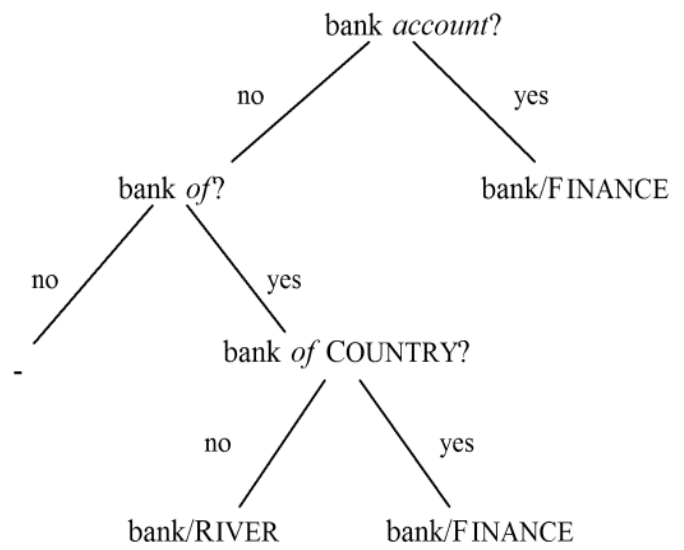
\includegraphics[width=0.5\textwidth]{images/decisiontree}
	\caption[Step-by-step deletion of neighbours]{Step-by-step deletion of neighbours}
	\label{fig:roothubdetection}
\end{figure}

A decision tree denotes classification rules in the form of a tree structure that recursively divides the training data set. Internal nodes of the decision tree denote a test which is going to be applied on a feature value and each branch denotes an output of the test. When a leaf node is reached, the sense of the word is represented (if possible). Fig.1 illustrates an example of a decision tree. We use this tree to disambiguate the polysemous word “bank” in the sentence, “The fishermen walk on the bank of Amazon”. The tree takes the path of no-yes-no to end up at the leaf bank/RIVER which is the sense of the word ‘bank’ in the sentence. Empty value of leaf node says that no selection is available for that feature value. 

Generating training data manually requires lot of manual efforts plus the data
can’t be trusted on its accuracy. Since the training data does not have the inputs
classified correctly, this can result in getting wrong disambiguated results

\subsection{Unsupervised Learning Approach}
In Unsupervised learning method it tries to find hidden structure in
unlabeled data. Unsupervised methods for WSD can be broadly divided into two
categories namely vector clustering-based and graph based ones. For graph based
methods generally unsupervised approach is preferred since it offers an
advantage of not requiring the training data.
Clustering – finding natural groupings of items. According to Markov clustering algorithm, considering a graph, there will be many links within a cluster, and fewer links between clusters. This means if you were to start at a node, and then randomly travel to a connected node, you’re more likely to stay within a cluster than travel between clusters.

Unsupervised WSD [53-55] methods do not depend on external knowledge sources or sense inventories, machine readable dictionaries or sense-annotated data set. According to Veronis, 2004 one of the main problems in word sense disambiguation lies in the very sense lists used by the systems. Conventional dictionaries are not suited to this task as they usually contain definitions that are too general.  For this reason instead of assigning the meaning to the words from the existing knowledge sources, unsupervised approaches deduce the word meanings based on information, found in raw corpora. This is called Word Sense Induction.

There are two main models proposed in the literature for
representing words:
• The vector space model, where words are represented as
a vector of features and the result is a cluster of similar
words, for each word to disambiguate. Each word is represented by a vector in a high-dimensional space. The dimensions of the space are the different words that can occur in context with any word in the corpus, and the value of each component of the vector is the number of cooccurrences in a given context window. Consider the two word senses of the french word \textit{barrage} which are \textit{eau}(water) and \textit{match}(match or game). Fig. 1 shows the corresponding vector in a two-dimensional space. However, using the vector-based techniques , large frequency 

• The graph space model, where words are represented
by cooccurance graphs and the relationships between words are represented by  weighted edges. The weight of an edge can be
computed either proportionally to the number of co-
occurrence between the words connected [8] or by means
of similarity measures. An
advantage of this approach is that it models relationships
between words, rather than words in isolation. This
way, it tends to better detect low-frequency senses of
ambiguous words

Hyperlex is one of the graph-based word sense induction techniques proposed by Venois. 



\newpage
\section{Hyperlex}
Hyperlex is an excellent graph based unsupervised approach that is capable of automatically determining word uses in a textbase without recourse to a dictionary. The algorithm makes use of the specific properties of word co-occurance graphs, which are shown as having small-world properties. The small-world nature of a graph can be explained in terms of its clustering coefficient and characteristic path length. The clustering coefficient of a graph shows the extent to which nodes tend to form connected groups that have many edges connecting each other in the group, and few edges leading out of the group. On the other side, the characteristic path length represents “closeness” in a graph. Randomly built graphs exhibit low clustering coefficients and are believed to represent something very close to the minimal possible average path length, at least in expectation. Perfectly ordered graphs, on the other side, show high clustering coefficients but also high average path length. According to Watts and Strogatz (1998), small-world graphs lie between these two extremes: they exhibit high clustering coefficients, but short average path lengths.

HyperLex algorithm accepts a collection of sentences including the target word as an input. Then
it induces the senses of the target words as follows: (1) create a co-occurrence graph whose
nodes are words in the context of the target word, (2) the nodes which
represents the sense, called ‘hub’, are identified, (3) the graph is subdivided into several
sub-trees whose root nodes are the identified hubs, (4) and finally a sense of a word in a new context is disambiguated using the sub-trees. The detail of each step will be described in the
following sections.

\subsection{Building cooccurance graphs}

Hyperlex depends on two most important charecterestics of to extract sense from words. They are frequency and Co-occurance. Frequency is the number of times a word occurs in the text corpora. A target word is said to cooccur with another word if they both appear in the same context. The cooccurance count is the number of times the two words cooccur in the corpora. These two parameters form the basis of calculating weights of the edges of the graph. 

Only nouns and adjectives are considered to be the target words for disambiguation as including verbs causes a notable decline in performance since too many verbs like \textit{can} and \textit{start} have very general uses and they tend to cooccur with lot of words and do not help in the disambiguation process. Words with less than 10 occurances in the entire subcorpus should be discarded. Contexts containing fewer than 4 words after filtering should be deleted and only those cooccurances with a cooccurance count of 5 or should be retained.

A graph G(V,E) is constructed for every target word that is to be disambiguated with all the cooccuring words as the vertices V. The edges of the graph depend on whether the cooccuring words of the target word are cooccuring themselves. 

The edges of the graph are assigned weights which depends on the frequency of the connecting words and the cooccurance count. The weight decreases as the cooccurance count increases. It is calculated as

\textit{\[W_{A,B} =  1 - max[p(A|B),p(B|A)]\]}

where \textit{p(A|B)} denotes the conditional probability of observing A in a given context, knowing that context contains B, and inversely, \textit{p(B|A)} is the probability of observing B in a given context, knowing that it contains A. The probabilities depend on the frequencies of the individual words and the cooccurance count.
\textit{\[p(A|B) = f_{A,B}/f_B,\]}
\textit{\[p(B|A) = f_{B,A}/f_A\]}

Veronis implemented Hyperlex on ten highy polysemous words. Table 2 shows the number of contexts in which the word pairs \textit{eau - ouvrage} (water - work) and \textit{eau - potable}(water - drinkable) appear together or seperately in the \textit{barrage} subcorpus.\newline

\textit{p(eau|ouvrage) =} 183/479 = 0.38,\ \  \textit{p(ouvrage|eau) = } 183/1057 = 0.17,\ \    \textit{w} = 1 \textminus\  0.38 = 0.62.
\newline


\textit{p(eau|potable) = }63/63 = 1, \ \ \ \textit{p(potable|eau) = }63/1057 = 0.06, \ \ \  \textit{w = }1 \textminus\ 1 = 0.

The weight of the edge reflects the magnitude of the semantic distance between words. When the words always cooccur then the weight is equal to 0 and when the words never cooccur then the weight is 1. Edges with weight above 0.9 should be eliminated to make sure that only strong associations are included in the graph. Otherwise the graph tends to become totally connected as the corpus grows in size, due to accidental cooccurances of any word pairs.

 
  \ctable[
   caption = Number of cooccurances of eau-ouvrage(water-work) and eau-potable(water-drinkable),
    cap = Technical Data of the Mitsubishi i-MiEV,
    label   = tab:data_imiev,
    pos = htb,
    mincapwidth = \textwidth,
    width = \textwidth,
    left
    ]{lccc cccccccccccccccccccccccc   ccccrrr}
    {}
    {\FL    &&&&&&&&&  EAU &&&&&&&&& \textasciitilde EAU &&&&&&&&&  Total
        \ML OUVRAGE &&&&&&&&& 183 &&&&&&&&& 296 &&&&&&&&& 489
		\NN \textasciitilde OUVRAGE &&&&&&&&& 874 &&&&&&&&& 5556 &&&&&&&&& 6430        
		\NN &&&&&&&&& &&&&&&&&& &&&&&&&&&
        \NN Total &&&&&&&&&  1057 &&&&&&&&& 5822 &&&&&&&&& 6909
        \NN &&&&&&&&& &&&&&&&&& &&&&&&&&&
        \NN POTABLE &&&&&&&&&  63 &&&&&&&&& 0 &&&&&&&&& 63
        \NN \textasciitilde POTABLE &&&&&&&&&  994 &&&&&&&&& 5852 &&&&&&&&& 6846
        \NN  &&&&&&&&& &&&&&&&&& &&&&&&&&&
        \NN Total &&&&&&&&& 1057 &&&&&&&&& 5852 &&&&&&&&& 6909
        \LL}

\subsection{Detection of root hubs}

\begin{figure}[htb]
	\centering
	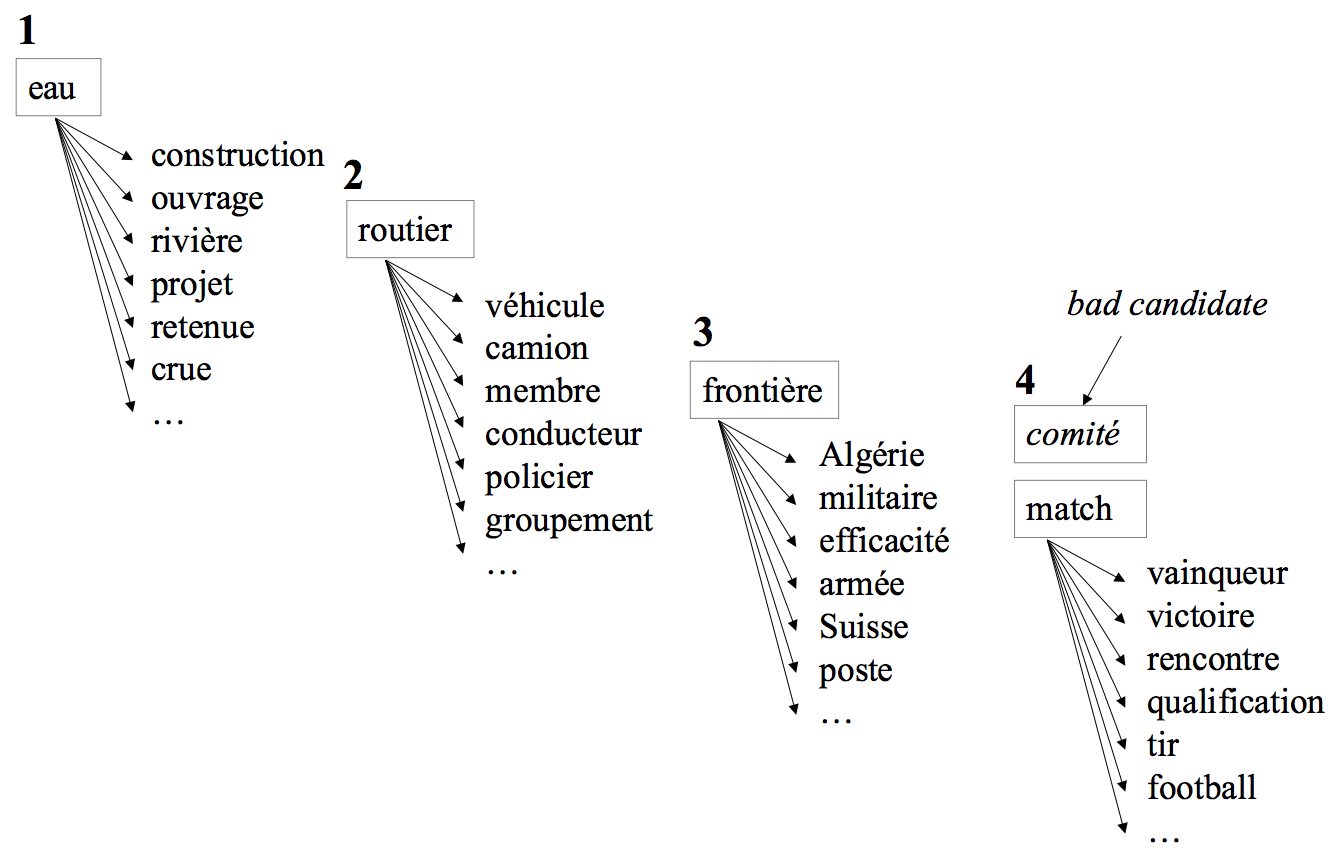
\includegraphics[width=150mm]{images/roothubdetectionclarity}
	\caption[Step-by-step deletion of neighbours]{Step-by-step deletion of neighbours}
	\label{fig:roothubdetection}
\end{figure}

\begin{algorithm}[H]
	
 \KwIn{\textit{G}: cooccurrence graph; \newline \textit{Freq}: array of frequencies of nodes in G}

 \textit{V} $\leftarrow$ array of nodes in G sorted in decreasing order of frequency\;
 \textit{H} $\leftarrow$ $\emptyset$\;
 \While{ \textit{V} $\neq$ $\emptyset$ \textbf{et} \textit{Freq(V[0])} < \textit{threshold}}{
  \textit{v} $\leftarrow$ \textit{V}[0]\;
  \If{GoodCandidate(\textit{v})}{
   \textit{H} $\leftarrow$ \textit{H} $\cup$ \textit{v}\;
   \textit{V} $\leftarrow$ \textit{V} \textminus \  (\textit{v} $\cup$ \textit{$\Gamma$}(\textit{v}))\;
   }
 }
 \textbf{return} \textit{H}
\end{algorithm}

\subsection{Delineating components}
\begin{figure}[htb]
	\centering
	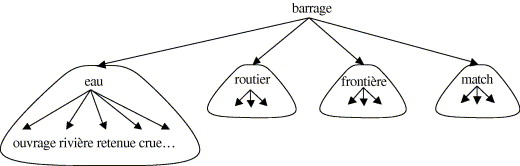
\includegraphics[]{images/delineate}
	\caption[Minimum spanning tree and high-density components.]{Minimum spanning tree and high-density components.}
	\label{fig:delineate}
\end{figure}


\begin{algorithm}[H]
	
 \KwIn{\textit{G}: cooccurrence graph; \newline \textit{H}: set of root hubs \newline \textit{t}: target word }

 \textit{G'} $\leftarrow$ \textit{G} $\cup$ \textit{t} \;
 
 \ForEach {$h  \in   H $}{
	add edge < \textit{t}, \textit{h} > with weight 0 to \textit{G'} 
 }
 \textit{T} $\leftarrow$ MST(\textit{G'}, \textit{t}) \newline
 \textbf{return} \textit{T}
\end{algorithm}

\subsection{Disambiguation}

\[ \mathbf{s_i} = \frac{1}{1 + \mathit{d}(\mathit{h_{i,v}})} \ \ \textrm{if \textit{v} belongs to component \textit{i},}\] 
\[ \mathbf{s_i} = 0 \ \ \textrm{otherwise.} \]

\begin{figure}[htb]
	\centering
	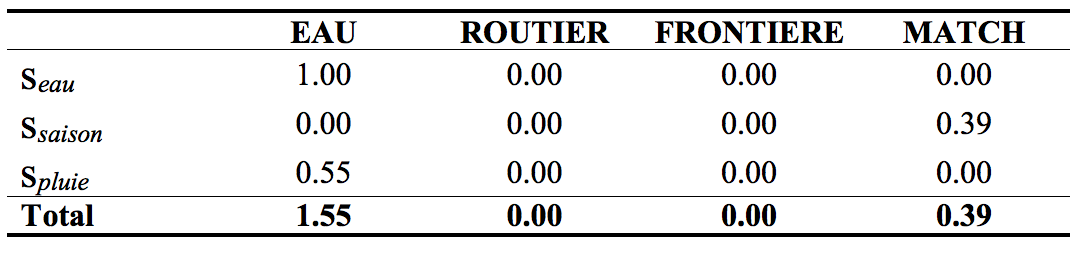
\includegraphics[width=90mm]{images/wsdscore}
	\caption[Minimum spanning tree and high-density components.]{Minimum spanning tree and high-density components.}
	\label{fig:delineate}
\end{figure}

\newpage
\section{Implementation details}
The implementation of the application is broken down into 5 phases
1. File Processing
2. First level (hashing)
3. Second Level
4. Graph processing
5. Disambiguation
\newpage
\subsection{Input data and conll files}
The application is run on a cluster with varying number of cores and data to get the expermental results for strong scaling weak scaling and we assume that the application is scalable upto terabytes of input data. The input data for the application are conll format[link to conll paper] files which is shown in the figure ... Each sentence is assigned an id. The words in each sentence are annotated with their lemma or base word and their parts of speech.  As mentioned in the hyperlex paper only the adjectives and nouns are considered for disambiguation and all the words which are occuring less than 10 times in the whole data are removed and the ones which are co-occuring less than 5 times are also not considered.

\newpage
\subsection{File Processing}
MPI IO provides simultaneous parallel access to a file by a group of processes.  The basic MPI::File::seek and MPI::File::read function work much like their unix counterparts. They are independent operations that use local file pointers to determine where in the file to access data for each process. While reading the files the processes a chunk of data from the file with broken sentences or incomplete sentences on either side of the data. we fixed this by sending the broken sentences to the corresponding processes. Once the processes have all complete sentences they proceed for processing the data, in which they extract the words along with their parts of speech, their frequency and their co-occuring words.

\centering

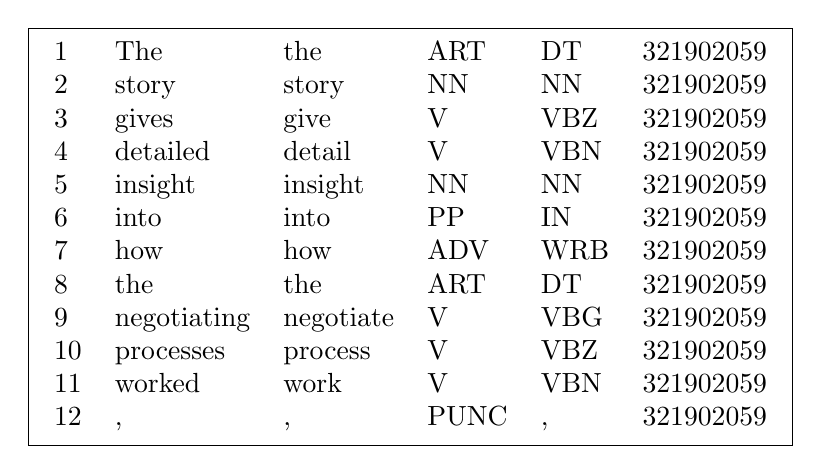
\begin{tikzpicture}
        \node[draw] {\begin{tabular}{l l l l l l}
      1&The&the&ART&DT&321902059 \\
2&story&story&NN&NN&321902059\\
3&gives&give&V&VBZ&321902059\\
4&detailed&detail&V&VBN&321902059\\
5&insight&insight&NN&NN&321902059\\
6&into&into&PP&IN&321902059\\
7&how&how&ADV&WRB&321902059\\
8&the&the&ART&DT&321902059\\
9&negotiating&negotiate&V&VBG&321902059\\
10&processes&process&V&VBZ&321902059\\
11&worked&work&V&VBN&321902059\\
12&,&,&PUNC&,&321902059\\
     \end{tabular}   };
    \end{tikzpicture}
   
   

\begin{figure}[htb] 

\subfloat{
\centering
\resizebox{0.5\textwidth}{!}{% 
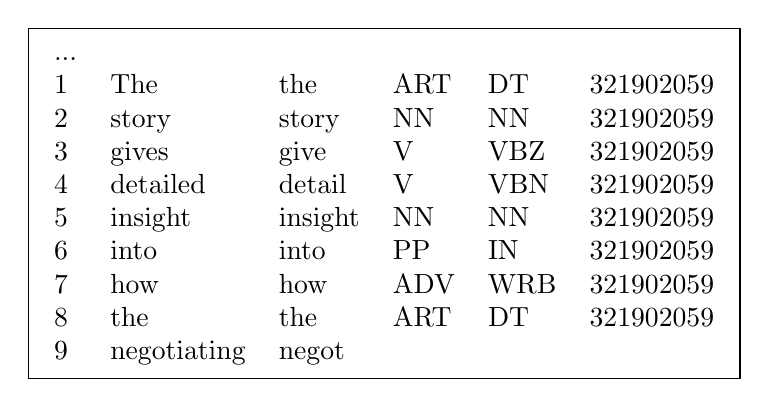
\begin{tikzpicture}
        \node[draw] {\begin{tabular}{l l l l l l}
        ...&&&&&\\
      1&The&the&ART&DT&321902059 \\
2&story&story&NN&NN&321902059\\
3&gives&give&V&VBZ&321902059\\
4&detailed&detail&V&VBN&321902059\\
5&insight&insight&NN&NN&321902059\\
6&into&into&PP&IN&321902059\\
7&how&how&ADV&WRB&321902059\\
8&the&the&ART&DT&321902059\\
9&negotiating&negot
     \end{tabular}   };
    \end{tikzpicture}}%
 }



\subfloat{
\centering
\resizebox{0.5\textwidth}{!}{%
   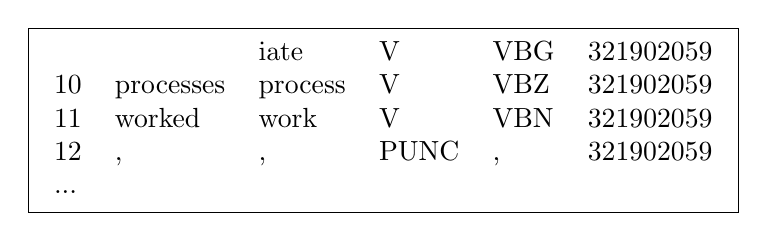
\begin{tikzpicture}
        \node[draw] {\begin{tabular}{l l l l l l}
     &&iate&V&VBG&321902059\\
10&processes&process&V&VBZ&321902059\\
11&worked&work&V&VBN&321902059\\
12&,&,&PUNC&,&321902059\\
...&&&&&
     \end{tabular}   };
    \end{tikzpicture}
    }%
    }
\caption{This figure has a width which is a factor of text width}

\end{figure}
   

\begin{figure}[htb]
	\centering
	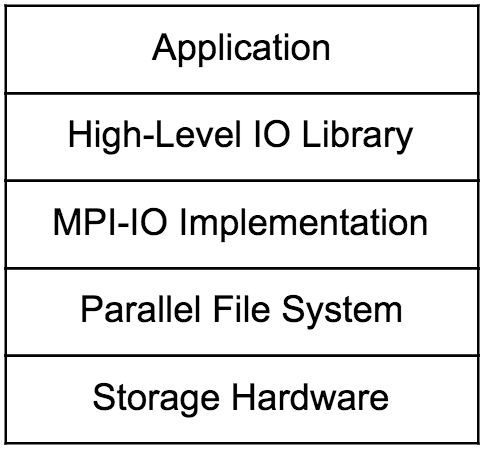
\includegraphics[width=0.3\textwidth]{images/paralleliostack}
	\caption[Hash Distribution]{Hash Distribution}
	\label{fig:paralleliostack}
\end{figure}

    – High-level I/O library maps application abstractions to a structured, portable file format (e.g., HDF5, Parallel netCDF)
– Middleware layer deals with organizing access by many processes (e.g., MPI-IO, UPC-IO) – Parallel file system maintains logical file space, provides efficient access to data (e.g., Lustre, PVFS, GPFS)    
    
    


\begin{figure}[htb]
	\centering
	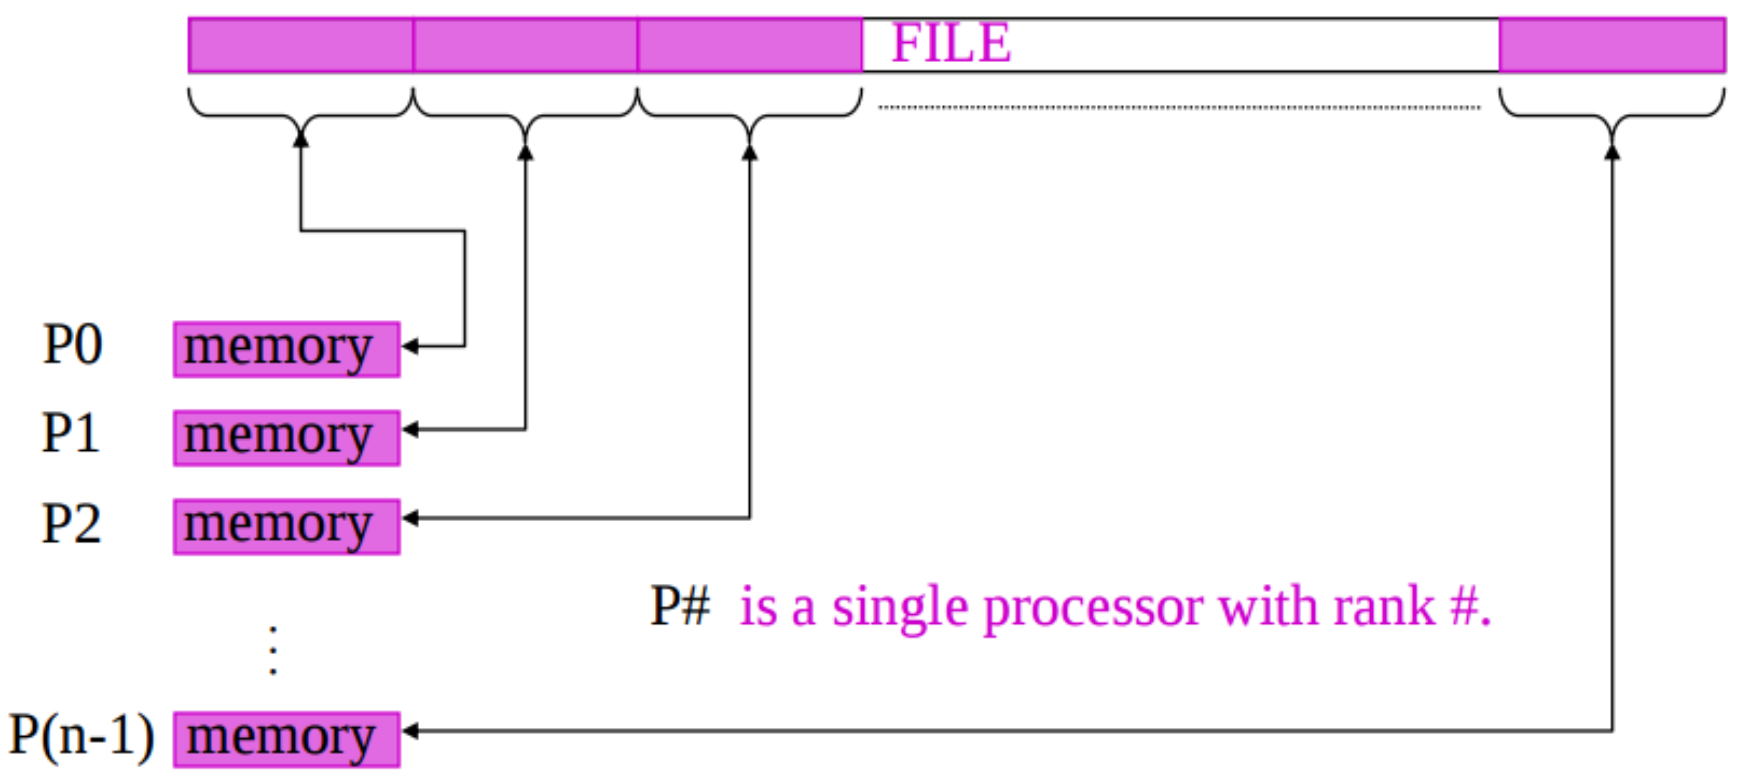
\includegraphics[width=150mm]{images/fileprocessing}
	\caption[Step-by-step deletion of neighbours]{Step-by-step deletion of neighbours}
	\label{fig:fileprocessing}
\end{figure}


\newpage
\subsection{Compression and Decompression}
In order to reduce memory latency, the files are read only once and stored in compressed format in the memory. So that they can be retrieved faster and worked upon. The files are compressed by upto 2%.

\newpage
\subsection{First level}
After the initial processing of the data that is read from the files, it so happens that the same words are present in multiple process with partial attribute data like frequency and the co-occuring words. To continue to further processing each word along with all its attribute data must be present in a single process. Initially we broadcasted the words present in each process to every other process and in case the other processes has the same words they sent back the words attribute data and deleted that data in their memory. And this was done linearly from process with rank 0 to n-1. But this resulted in an uneven distribution of data where the first few processes contained large amounts of data and it declined exponentially towards the last process. We bettered this approach by doing in a round robin fashion instead of doing it linearly and by sending only a pre-determined amount of words at a time. But this approach was much inefficient as it increased the amount of communication involved between the processes and thereby increasing the time taken to process.

Keeping in mind, the amount of communication involved between processes and an even distribution of data, we came up with a hash distribution technique where we assign a word to a process depending on their hash value. We calculate the hash of the word string and divides it with MPI communicator size 'n-1' and the remainder is the processes rank which is responsible for this word. Each process can individually calculate the hash for the words they have and send them to the process which is responsible for that word, resulting in a push mechanism where the communication is reduced by half. Fig. ... shows the distribution of the number of words among various processes and it shows that it is almost an even distribution of data.


\begin{figure}[htb]
	\centering
	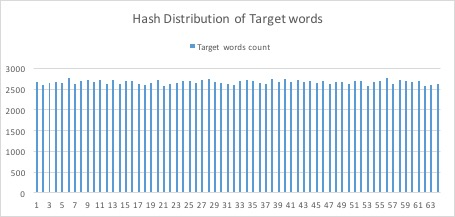
\includegraphics[width=0.7\textwidth]{images/hashdistribution}
	\caption[Hash Distribution]{Hash Distribution}
	\label{fig:hashdistribution}
\end{figure}



\newpage
\subsection{Second level}
To form a graph for a target word, we need all the co-occuring words(first level words) and also the edges between the co-occuring words. There is an edge between two co-occuring words only if the two words are co-occuring themselves. So we need to get the co-occuring words(second level words) of the co-occuring words of the target word to be able to construct a graph.

\begin{figure}[htb]
	\centering
	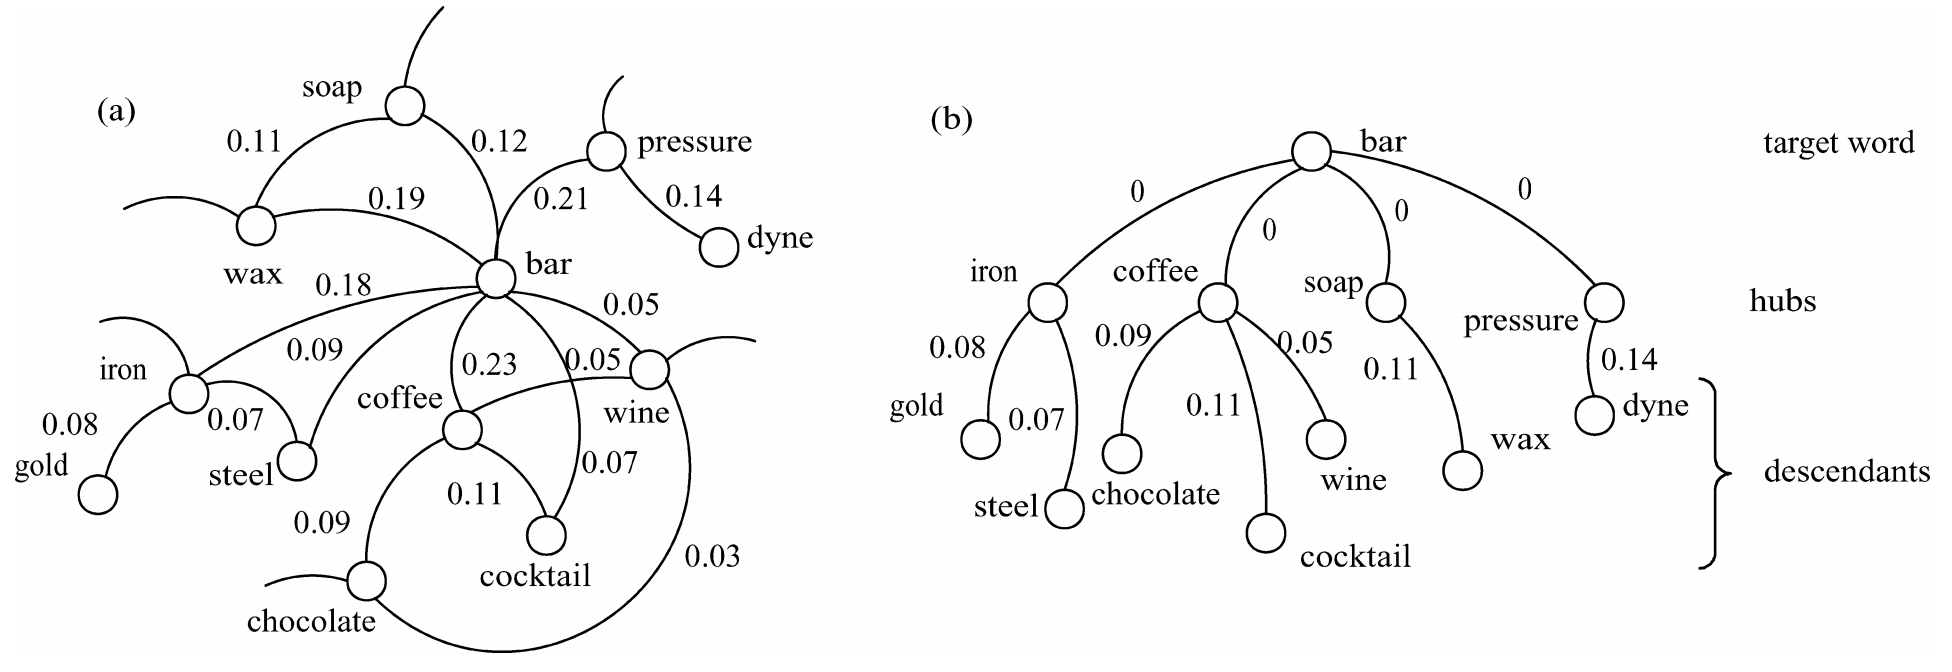
\includegraphics[width=150mm]{images/mst}
	\caption[Hash Distribution]{Hash Distribution}
	\label{fig:mst}
\end{figure}

\begin{figure}[h]
	\centering
	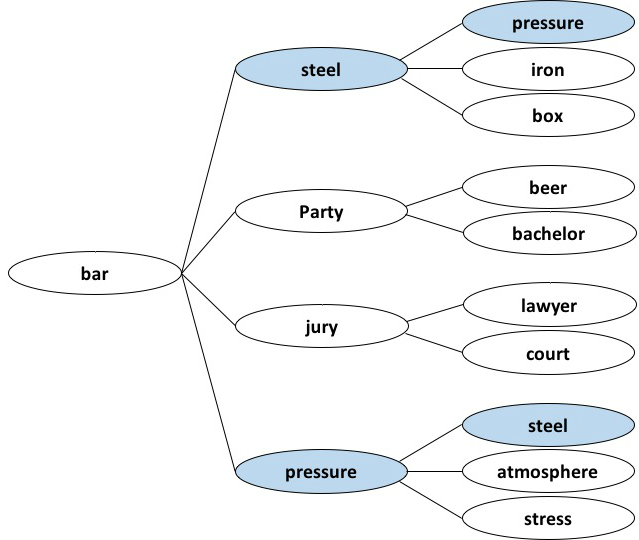
\includegraphics[width=0.4\textwidth]{images/secondlevel}
	\caption[Hash Distribution]{Hash Distribution}
	\label{fig:secondlevel}
\end{figure}



\newpage
\subsection{Graph Creation and WSI}
Once we have the data regarding the first level words along with all the edges between these words, we construct the graph and the roothubs are extracted from the graph. The roothubs are the words which are more frequently co-occuring with the target word. These root hubs form the word senses of the target word. Once we extract the root hubs, we perform an MST on the graph to delineate the words(in other words to align each word to its corresponding roothub), and the distance from itself to its corresponding roothub becomes its score which is later used in disambiguation phase.


\newpage
\subsection{Disambiguation}

The 

\newpage
\subsection{Experiment results}
\subsubsection{File Processing times}
\begin{figure}[!htb]
	\centering
	\subfloat[Strong Scaling]{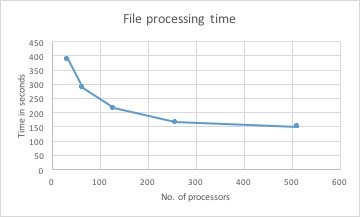
\includegraphics[width=80mm]{images/fileprocessingstrong}}\hspace{10mm}
	\subfloat[Weak Scaling]{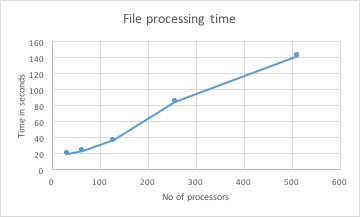
\includegraphics[width=80mm]{images/fileprocessingweak}	}
	\caption[File Processing Times]{File Processing Times}
	\label{fig:fileprocessing}
\end{figure}

\subsubsection{Target words distribution}
\begin{figure}[!htb]
	\centering
	\subfloat[Strong Scaling]{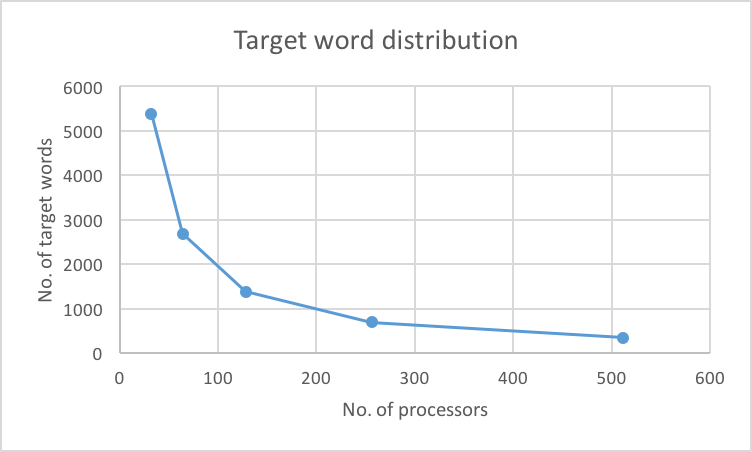
\includegraphics[width=80mm]{images/tdiststrong}}\hspace{10mm}
	\subfloat[Weak Scaling]{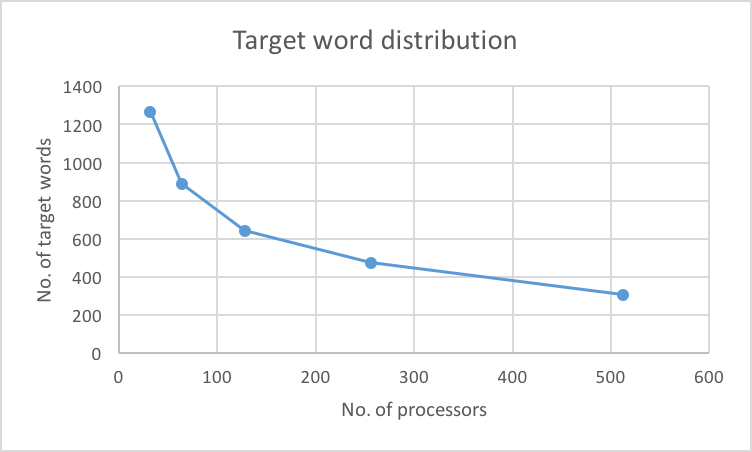
\includegraphics[width=80mm]{images/tdistweak}	}
	\caption[Target words distribution]{Target word distribution}
	\label{fig:targetworddist}
\end{figure}

\subsubsection{Compression and Decompression times}
\begin{figure}[!htb]
	\centering
	\subfloat[Strong Scaling]{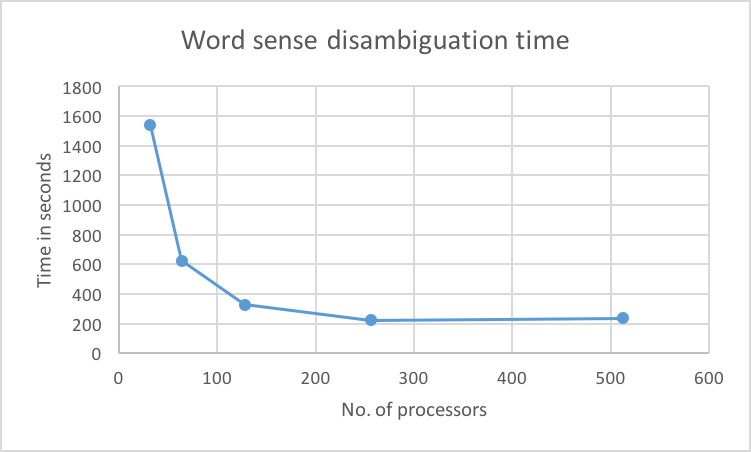
\includegraphics[width=80mm]{images/compdecompstrong}}\hspace{10mm}
	\subfloat[Weak Scaling]{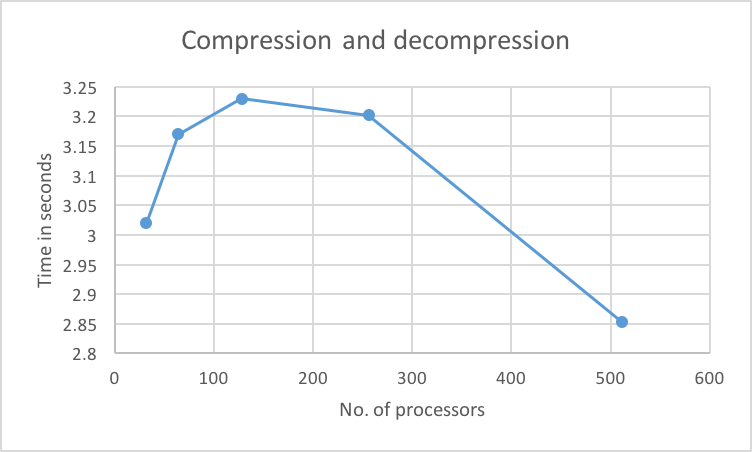
\includegraphics[width=80mm]{images/compdecompweak}	}
	\caption[Compression and Decompression Times]{Compression and Decompression Times}
	\label{fig:compdecomp}
\end{figure}
\newpage

\subsubsection{First Level times}
\begin{figure}[!htb]
	\centering
	\subfloat[Strong Scaling]{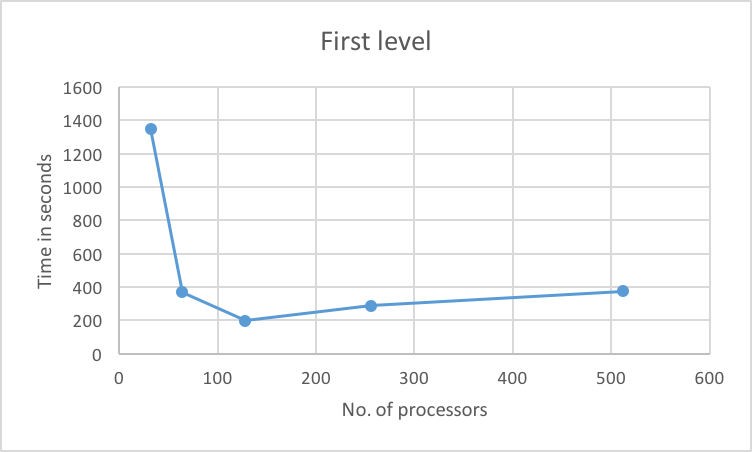
\includegraphics[width=80mm]{images/firstlevelstrong}}\hspace{10mm}
	\subfloat[Weak Scaling]{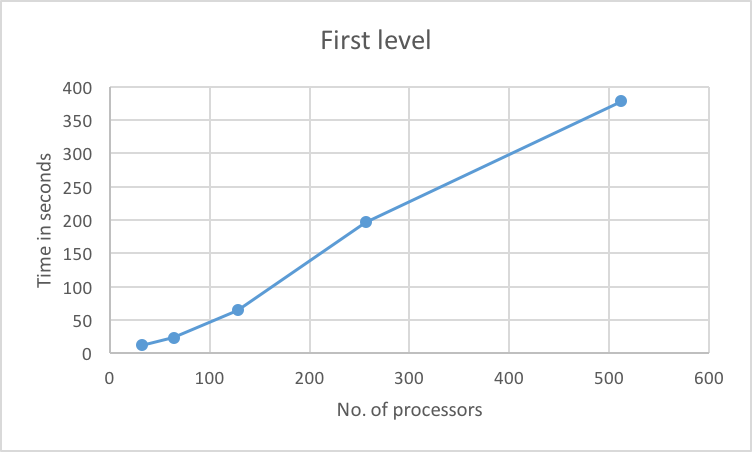
\includegraphics[width=80mm]{images/firstlevelweak}	}
	\caption[First Level Times]{First Level Times}
	\label{fig:compdecomp}
\end{figure}

\subsubsection{Second level and graph times}
\begin{figure}[!htb]
	\centering
	\subfloat[Strong Scaling]{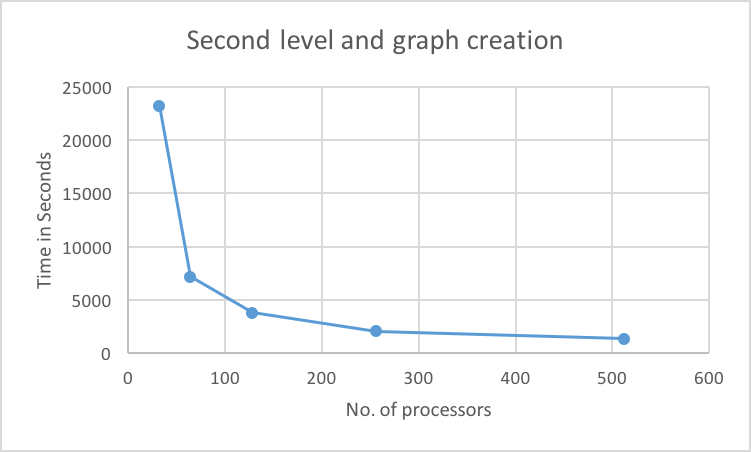
\includegraphics[width=80mm]{images/secondlevelstrong}}\hspace{10mm}
	\subfloat[Weak Scaling]{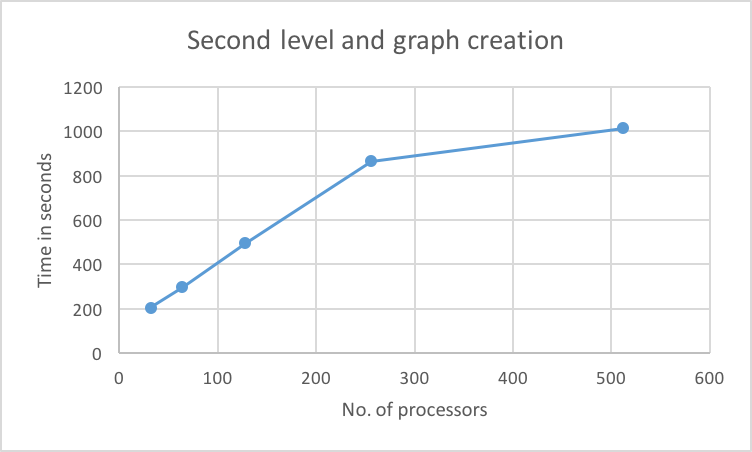
\includegraphics[width=80mm]{images/secondlevelweak}	}
	\caption[Compression and Decompression Times]{Compression and Decompression Times}
	\label{fig:compdecomp}
\end{figure}

\subsubsection{Disambiguation times}
\begin{figure}[!htb]
	\centering
	\subfloat[Strong Scaling]{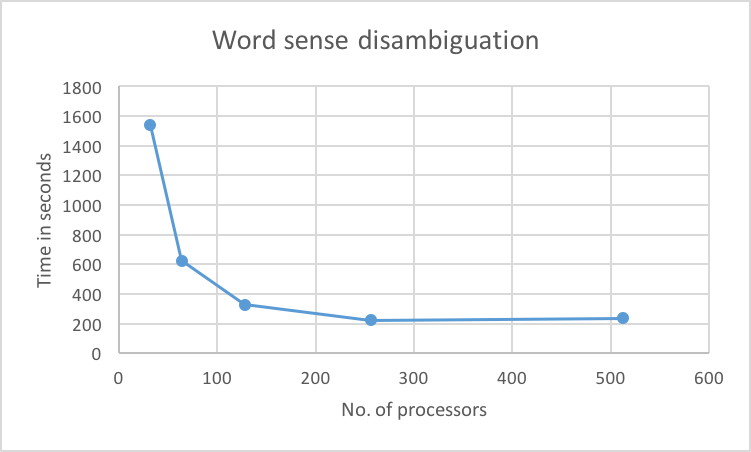
\includegraphics[width=80mm]{images/wsdstrong}}\hspace{10mm}
	\subfloat[Weak Scaling]{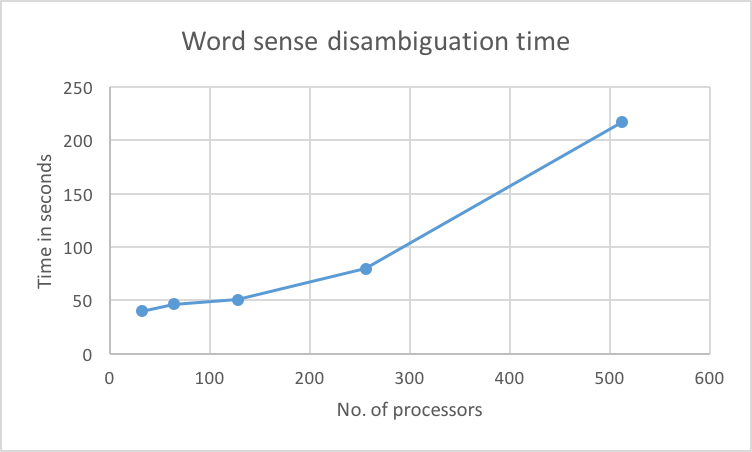
\includegraphics[width=80mm]{images/wsdweak}	}
	\caption[Disambiguation Times]{Disambiguation Times}
	\label{fig:compdecomp}
\end{figure}

\subsubsection{Total times}
\begin{figure}[!htb]
	\centering
	\subfloat[Strong Scaling]{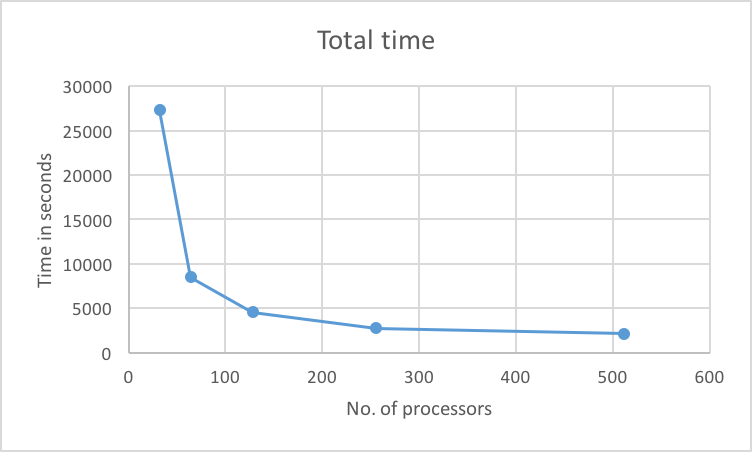
\includegraphics[width=80mm]{images/totaltimestrong}}\hspace{10mm}
	\subfloat[Weak Scaling]{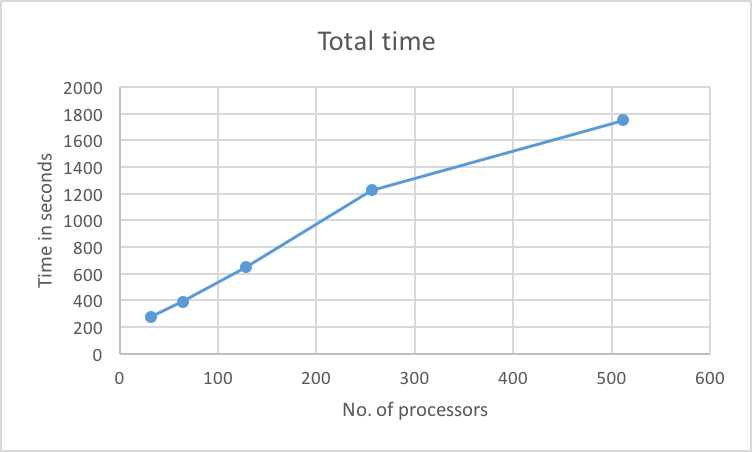
\includegraphics[width=80mm]{images/totaltimeweak}	}
	\caption[Total Times]{Total Times}
	\label{fig:compdecomp}
\end{figure} 

\section{Conclusion and Future work}
1. 

\section{bibliography}
 

\end{document}
